\section{Exercise 3: Stand-alone capacitor impedance poltting and validation}

%%%%%%%%%%%%%%%%%%%%%%%%%%%%%%%%%%%%%%%%%%%%%%%%%%%%%%%%%%%

\subsection{Extraction of capacitor impedance from vendor S-parameters}

The stand-alone impedance of the six candidate capacitors has been characterised in MATLAB starting from frequency-domain measurements given by the vendor.\\
The data are provided in the IdEM workspace \texttt{capacitors\_workspace.idem.mat}, which contains the MATLAB structure \texttt{idemws}. 
Its field \texttt{idemws.DUM} is a $6 \times 1$ cell array, one entry per capacitor, each storing:
\begin{itemize}
    \item  Part name, 
    \item  Vector of 401 logarithmically spaced frequency points,
    \item  The S-parameter matrix for each frequency point, stored as a $2 \times 2$ cell array of complex vectors,
    \item  The reference impedance $R_0 = 50~\Omega$.
\end{itemize}

The core extraction loop of the MATLAB script \texttt{cap\_impedance\_matlab.m} is shown below.

\begin{lstlisting}[language=Matlab, caption={Extraction of the stand-alone capacitor impedance from vendor S-parameters in \texttt{cap\_impedance\_matlab.m}.}, label={lst:capzextract}]
for k = 1:N
    D       = idemws.DUM{k};
    name{k} = D.Name;
    f{k}    = D.f(:);
    S21     = D.S{2,1}(:);
    Z{k}    = 2*D.R0*(1 - S21) ./ S21;
    C_nF(k) = str2double(D.Name(11:12)) * 10^str2double(D.Name(13)) * 1e-3;
end
\end{lstlisting}

\noindent The vendor characterised each component in \textit{series mode}, placing the capacitor in series between port~1 and port~2 of a two-port $R_0 = 50~\Omega$ measurement setup.\\
Under this configuration, the transmission parameter $S_{21}$ is related to the series impedance $Z$ of the capacitor by
\begin{equation}
    S_{21} = \frac{2 R_0}{Z + 2 R_0} \quad \Longrightarrow \quad Z = 2 R_0 \frac{1 - S_{21}}{S_{21}}.
    \label{eq:s21toz}
\end{equation}

\noindent For each component, the nominal capacitance in nF is also automatically decoded from the capacitor part number.\\


\noindent The resulting impedance magnitudes $|Z(f)|$ are plotted on a log--log scale from $0.1~\text{MHz}$ to $10~\text{GHz}$ in \ref{fig:capzvendor}. 
As expected for real decoupling capacitors, each curve exhibits a capacitive behaviour ($|Z| \propto 1/f$) at low frequency, reaches a minimum $|Z|_{\min}$ (corresponding to the equivalent series resistance, ESR) at its self-resonance frequency $f_{\text{SRF}}$, 
and becomes inductive ($|Z| \propto f$) above $f_{\text{SRF}}$ due to the equivalent series inductance (ESL).

\begin{figure}[!h]
\centering
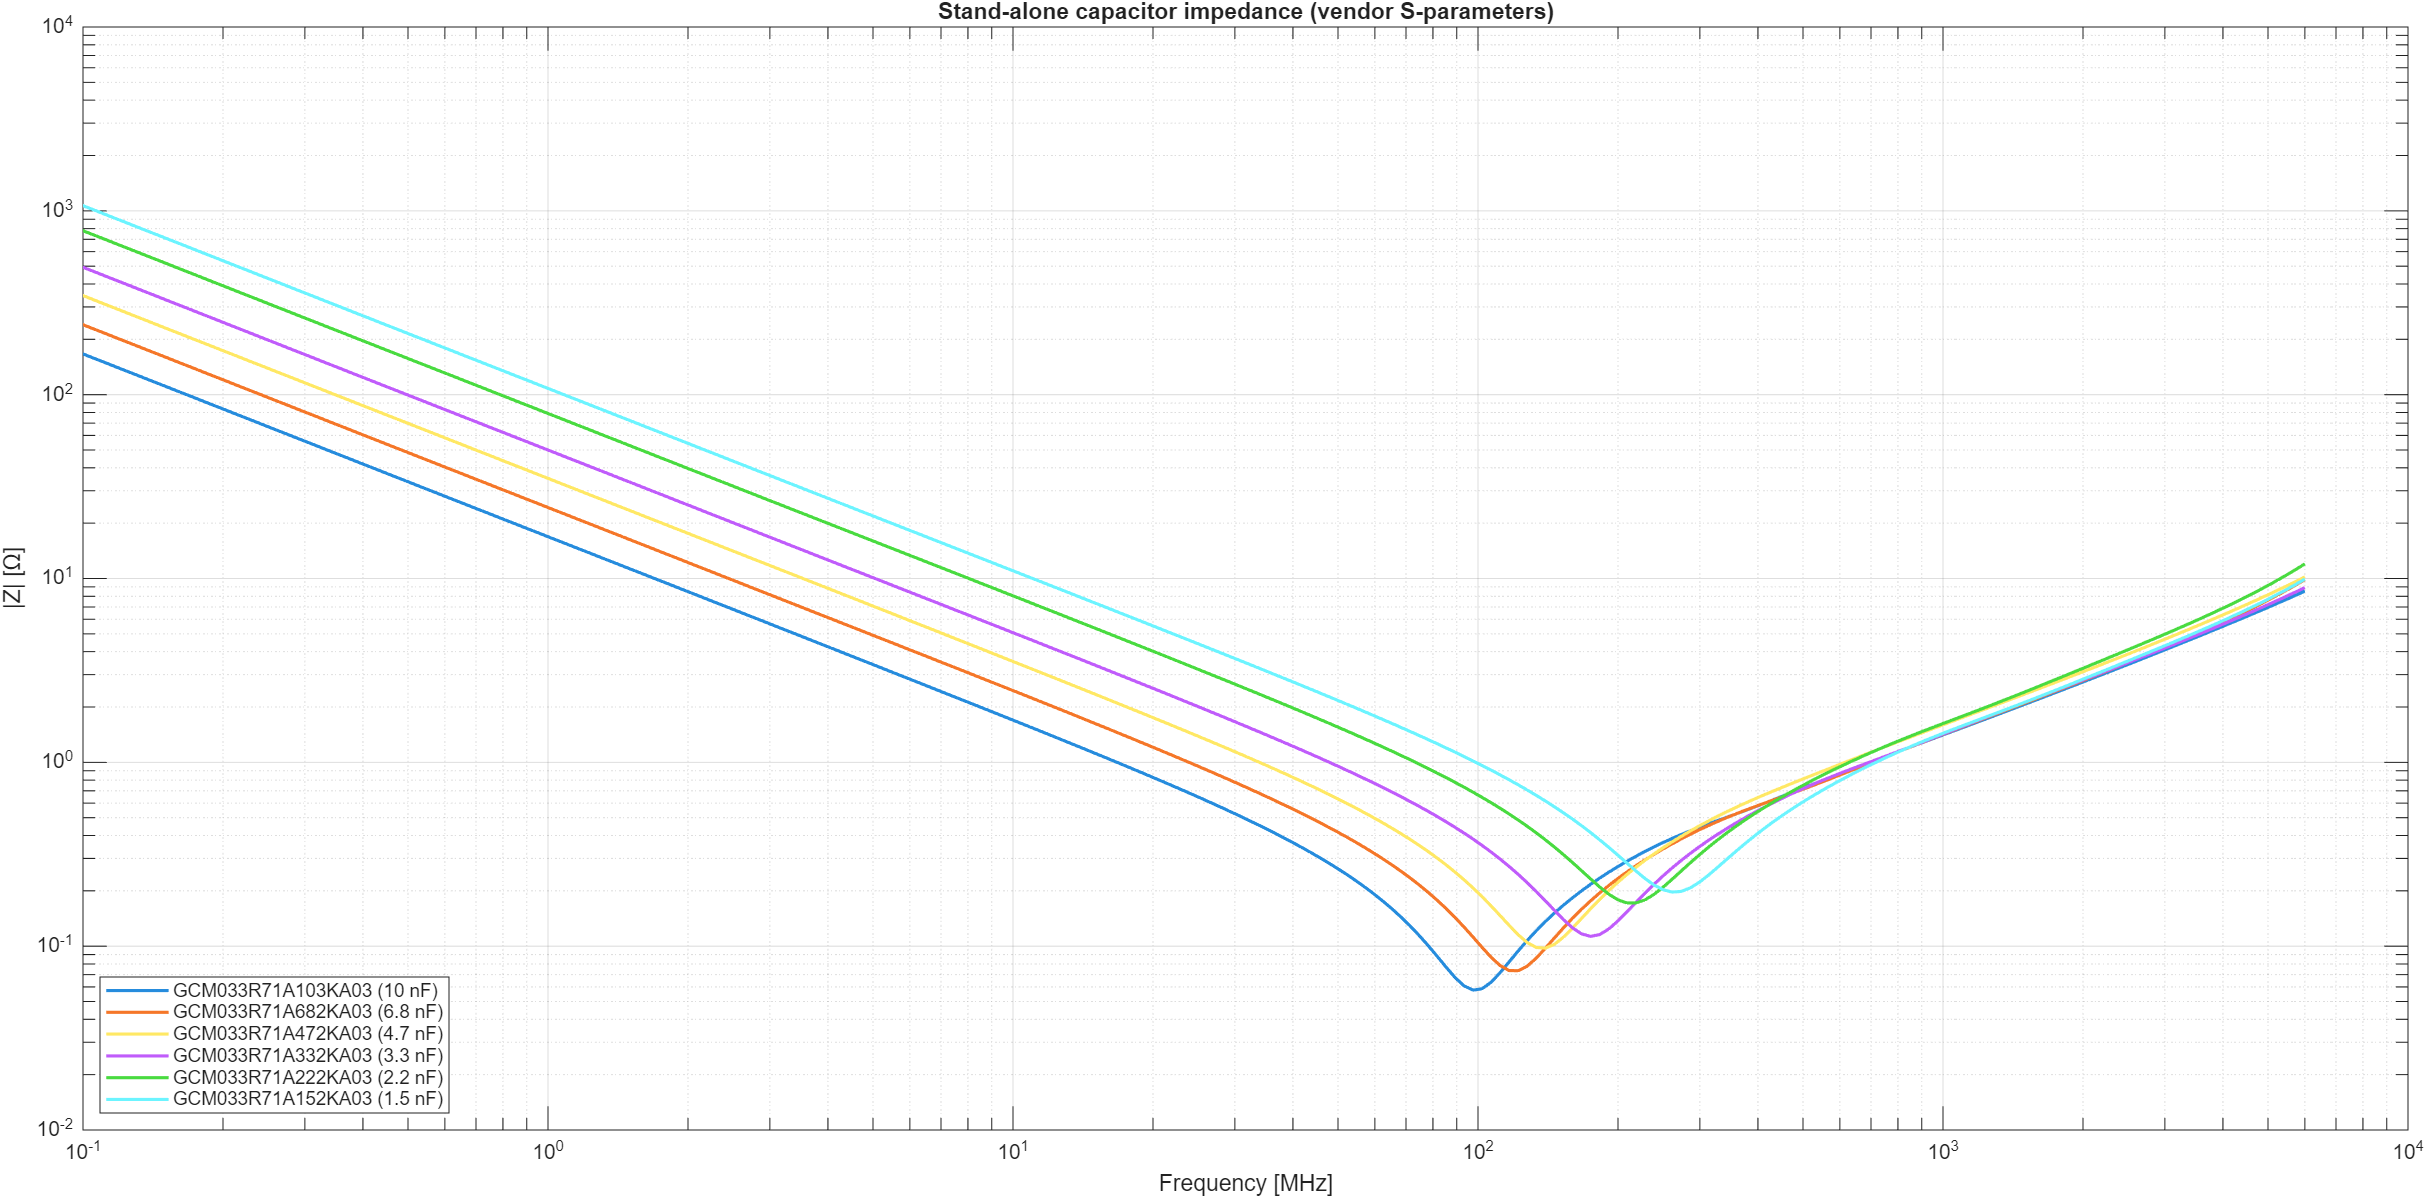
\includegraphics[width=0.7\textwidth]{./eser3/Images/caps.png}
\caption{Stand-alone impedance magnitude $|Z(f)|$ of the six Murata decoupling capacitors extracted from the vendor S-parameters.}
\label{fig:capzvendor}
\end{figure}

\noindent Table~\ref{tab:cap_srf} summarises the nominal capacitance, self-resonance frequency $f_{\text{SRF}}$, and minimum impedance $|Z|_{\min}$ extracted on the vendor frequency grid. It should be noted that the vendor grid consists of 401 logarithmically spaced points (approximately $4.6\%$ spacing per step), which sets the resolution limit on the extracted $f_{\text{SRF}}$ values. Finally, the extracted data (\texttt{f}, \texttt{Z}, \texttt{name}, \texttt{C\_nF}) are saved to \texttt{cap\_Z\_vendor\_data.mat} for the subsequent SPICE validation.

\begin{table}[!h]
\centering
\caption{Nominal capacitance, self-resonance frequency, and minimum impedance of the six capacitors extracted from vendor S-parameters.}
\label{tab:cap_srf}
\begin{tabular}{lccc}
\hline
\textbf{Part number} & \textbf{$C$ [nF]} & \textbf{$f_{\text{SRF}}$ [MHz]} & \textbf{$|Z|_{\min}$ [$\Omega$]} \\
\hline
\texttt{GCM033R71A103KA03} & 10.0 &  97.54 & 0.0577 \\
\texttt{GCM033R71A682KA03} &  6.8 & 122.01 & 0.0735 \\
\texttt{GCM033R71A472KA03} &  4.7 & 139.55 & 0.0976 \\
\texttt{GCM033R71A332KA03} &  3.3 & 174.57 & 0.1131 \\
\texttt{GCM033R71A222KA03} &  2.2 & 218.37 & 0.1717 \\
\texttt{GCM033R71A152KA03} &  1.5 & 261.20 & 0.1970 \\
\hline
\end{tabular}
\end{table}

%%%%%%%%%%%%%%%%%%%%%%%%%%%%%%%%%%%%%%%%%%%%%%%%%%%%%%%%%%%

\subsection{Validation of the vendor SPICE models}

To verify that the SPICE subcircuit models provided by the vendor accurately reproduce the measured frequency-domain behaviour, 
an AC simulation has been performed in LTspice on a testbench netlist (\texttt{caps\_spice\_ac.cir}) containing the six capacitor models driven by unit AC current sources, 
so that each node voltage directly equals the capacitor impedance $Z(f)$. 
The simulated node voltages (\texttt{V(zXXX)}, where \texttt{XXX} is the three-digit capacitance code) have been exported from LTspice as a text file (\texttt{caps\_spice\_ac.txt}).
\noindent Because the SPICE simulation and the vendor S-parameters may be defined on different frequency grids, the comparison is restricted to the overlapping frequency range and the SPICE response is interpolated onto the vendor frequency points:
The relative magnitude error is computed as
    \begin{equation}
        \varepsilon_{|Z|}(f) = \frac{\big||Z_{\text{SPICE}}(f)| - |Z_{\text{vendor}}(f)|\big|}{|Z_{\text{vendor}}(f)|} \times 100\%;
    \end{equation}

\begin{figure}[!h]
\centering
 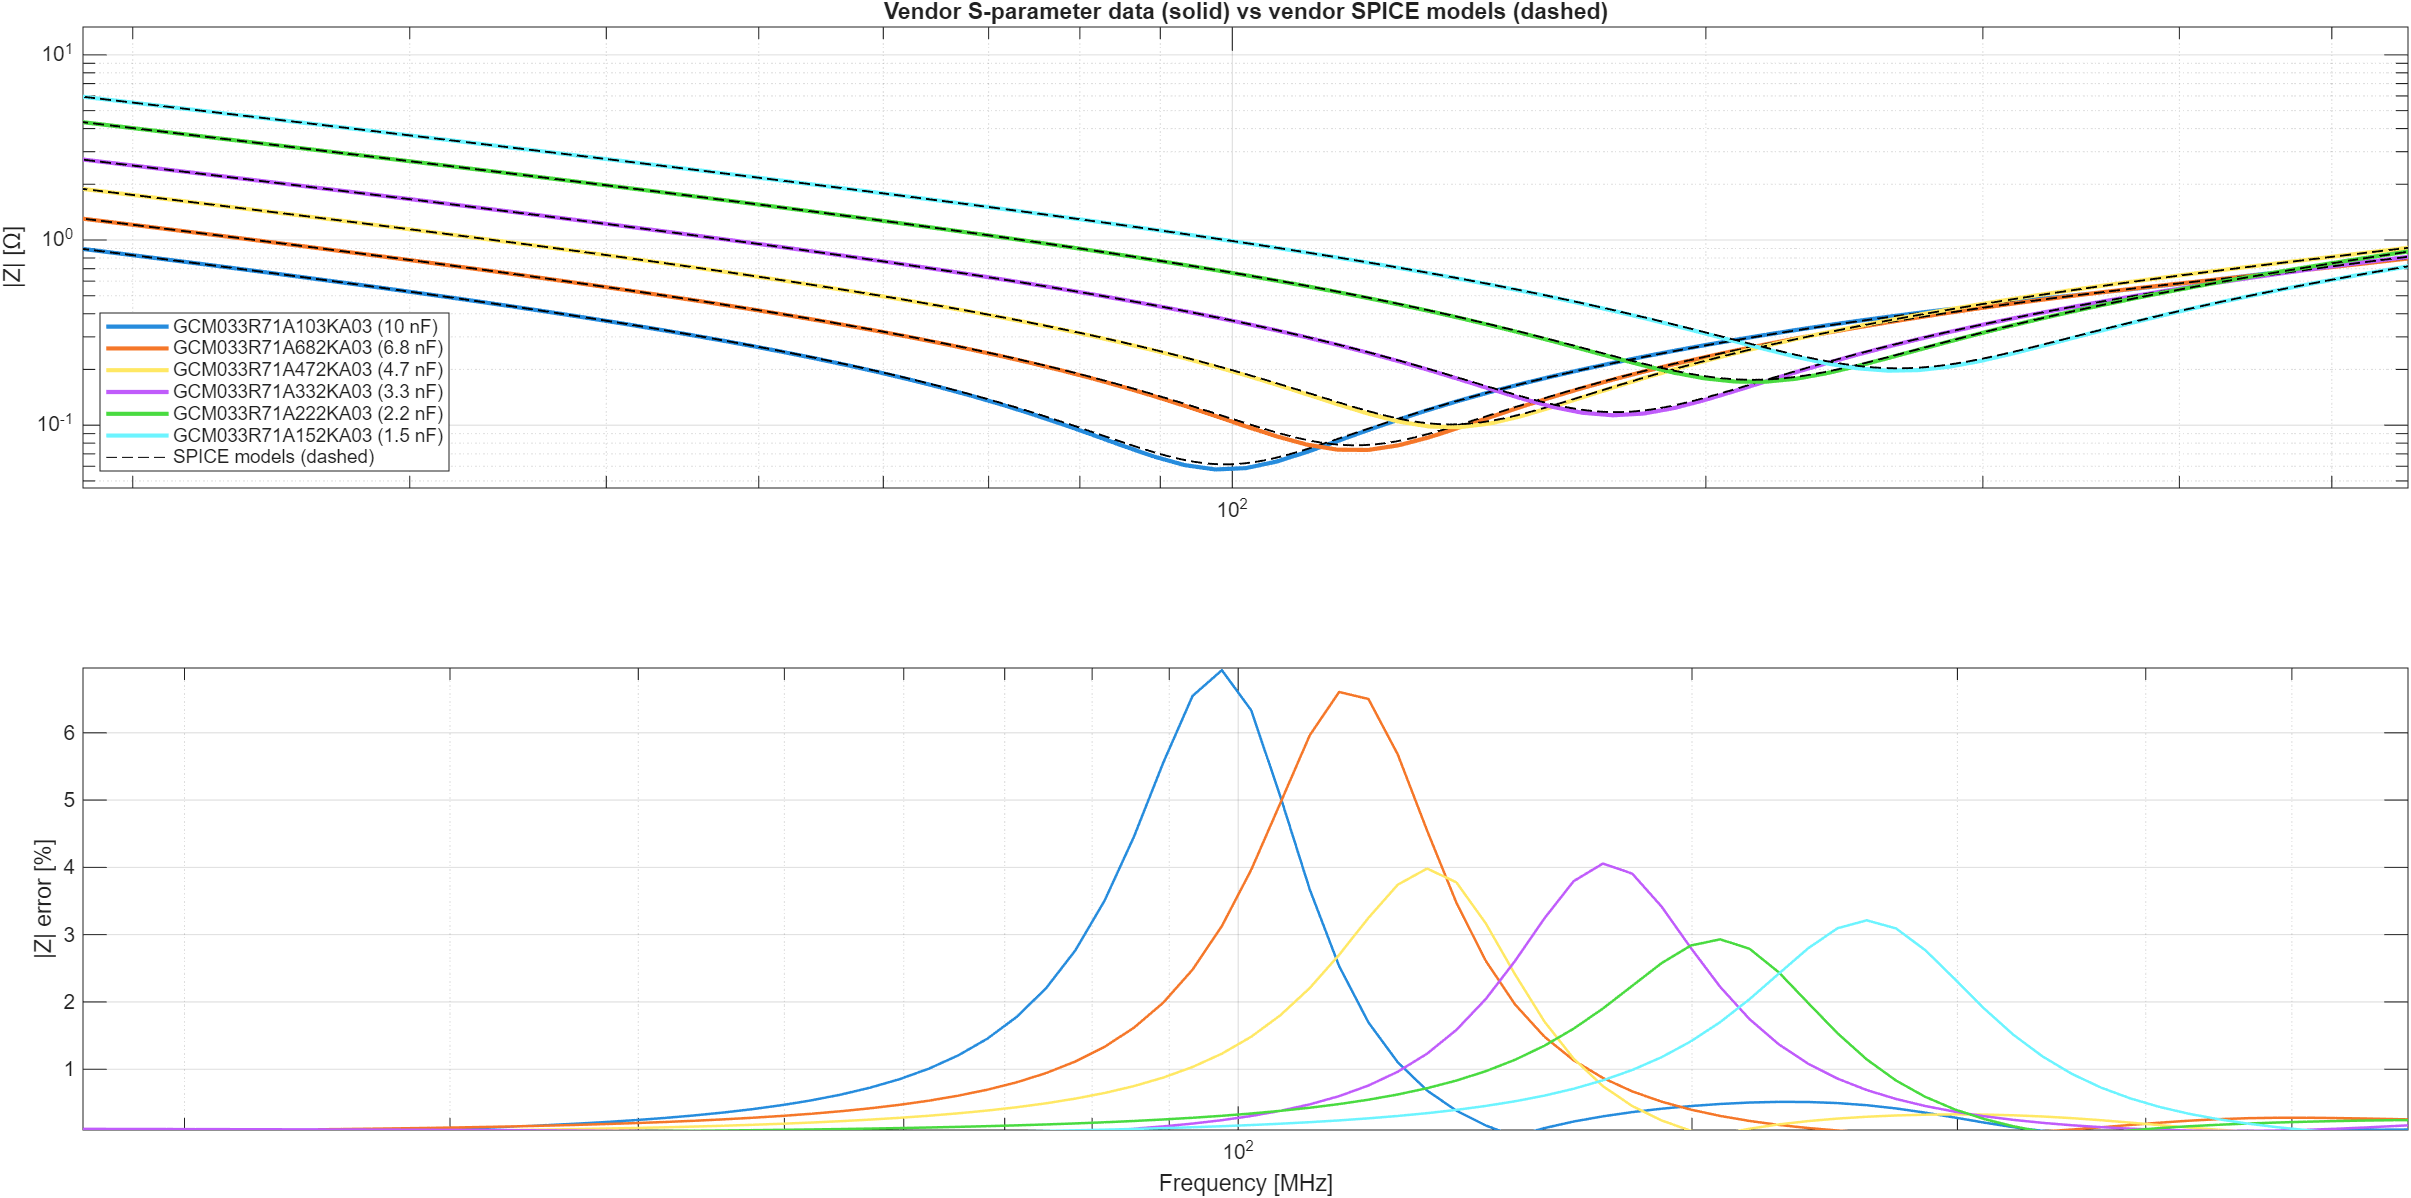
\includegraphics[width=0.92\textwidth]{./eser3/Images/cap_val.png}
\caption{Validation of the vendor SPICE models against the vendor S-parameter data. Top: impedance magnitude $|Z(f)|$ from vendor S-parameters (solid lines) and SPICE AC simulation (dashed black lines). Bottom: relative magnitude error $\varepsilon_{|Z|}$ versus frequency.}
\label{fig:capspiceval}
\end{figure}

\noindent The visual comparison between the vendor S-parameter curves and the SPICE simulations show a loss of accracy near the self-resonance frequency. 
This is confirmed by the relative magnitude error which peaks at the self-resonance frequency and is higher for bigger capacitors.

\begin{table}[!h]
\centering
\caption{Maximum impedance magnitude  between vendor S-parameters and vendor SPICE models.}
\label{tab:cap_val_err}
\begin{tabular}{lccc}
\hline
\textbf{Part number} & \textbf{Max $|Z|$ error [\%]} & \textbf{Frequency [MHz]} \\
\hline
\texttt{GCM033R71A103KA03} & 6.930 &  97.54   \\
\texttt{GCM033R71A682KA03} & 6.606 & 116.67   \\
\texttt{GCM033R71A472KA03} & 3.982 & 133.44   \\
\texttt{GCM033R71A332KA03} & 4.057 & 174.57   \\
\texttt{GCM033R71A222KA03} & 2.931 & 208.81   \\
\texttt{GCM033R71A152KA03} & 3.213 & 261.20   \\
\hline
\end{tabular}
\end{table}

\noindent Overall, the SPICE models show good agreement with the vendor S-parameter data across the frequency band of interest, 
confirming that they can be reliably used in the PDN simulations of the following exercises.